\subsection{Input handling}
To prevent multiple and unintended inputs from unstable button values, a debouncing routine is used to prevent signal propagation until a stable value can be acquired.

\begin{figure}[h]
    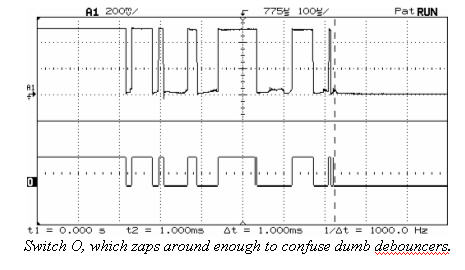
\includegraphics{figures/debounceswitcho.jpg}
    \caption{Illustration of unstable button behavior, taken from \cite{debouncer}}
\end{figure}
When a GPIO interrupt is received, the GPIO interrupt handler starts a debounce timer which will run for a predefined number of cycles, before turning itself off again.
The corresponding interrupt handler reads current  GPIO values, accepts them if the debouncing routine in listing \ref{lst:debounce} deems the input stable, and reject them otherwise.
If the input is accepted, the corresponding event is put in the queue of the FSM.

\lstinputlisting[caption={Debouncer, taken from \cite{debouncer}}, label={lst:debounce}, linerange={49-67}]{../code/buttons.c}

